\documentclass[12pt,a4paper]{article}

\usepackage[a4paper,text={16.5cm,25.2cm},centering]{geometry}
\usepackage{lmodern}
\usepackage{amssymb,amsmath}
\usepackage{bm}
\usepackage{graphicx}
\usepackage{microtype}
\usepackage{hyperref}
\setlength{\parindent}{0pt}
\setlength{\parskip}{1.2ex}

\hypersetup
       {   pdfauthor = { Marco Fasondini },
           pdftitle={ foo },
           colorlinks=TRUE,
           linkcolor=black,
           citecolor=blue,
           urlcolor=blue
       }




\usepackage{upquote}
\usepackage{listings}
\usepackage{xcolor}
\lstset{
    basicstyle=\ttfamily\footnotesize,
    upquote=true,
    breaklines=true,
    breakindent=0pt,
    keepspaces=true,
    showspaces=false,
    columns=fullflexible,
    showtabs=false,
    showstringspaces=false,
    escapeinside={(*@}{@*)},
    extendedchars=true,
}
\newcommand{\HLJLt}[1]{#1}
\newcommand{\HLJLw}[1]{#1}
\newcommand{\HLJLe}[1]{#1}
\newcommand{\HLJLeB}[1]{#1}
\newcommand{\HLJLo}[1]{#1}
\newcommand{\HLJLk}[1]{\textcolor[RGB]{148,91,176}{\textbf{#1}}}
\newcommand{\HLJLkc}[1]{\textcolor[RGB]{59,151,46}{\textit{#1}}}
\newcommand{\HLJLkd}[1]{\textcolor[RGB]{214,102,97}{\textit{#1}}}
\newcommand{\HLJLkn}[1]{\textcolor[RGB]{148,91,176}{\textbf{#1}}}
\newcommand{\HLJLkp}[1]{\textcolor[RGB]{148,91,176}{\textbf{#1}}}
\newcommand{\HLJLkr}[1]{\textcolor[RGB]{148,91,176}{\textbf{#1}}}
\newcommand{\HLJLkt}[1]{\textcolor[RGB]{148,91,176}{\textbf{#1}}}
\newcommand{\HLJLn}[1]{#1}
\newcommand{\HLJLna}[1]{#1}
\newcommand{\HLJLnb}[1]{#1}
\newcommand{\HLJLnbp}[1]{#1}
\newcommand{\HLJLnc}[1]{#1}
\newcommand{\HLJLncB}[1]{#1}
\newcommand{\HLJLnd}[1]{\textcolor[RGB]{214,102,97}{#1}}
\newcommand{\HLJLne}[1]{#1}
\newcommand{\HLJLneB}[1]{#1}
\newcommand{\HLJLnf}[1]{\textcolor[RGB]{66,102,213}{#1}}
\newcommand{\HLJLnfm}[1]{\textcolor[RGB]{66,102,213}{#1}}
\newcommand{\HLJLnp}[1]{#1}
\newcommand{\HLJLnl}[1]{#1}
\newcommand{\HLJLnn}[1]{#1}
\newcommand{\HLJLno}[1]{#1}
\newcommand{\HLJLnt}[1]{#1}
\newcommand{\HLJLnv}[1]{#1}
\newcommand{\HLJLnvc}[1]{#1}
\newcommand{\HLJLnvg}[1]{#1}
\newcommand{\HLJLnvi}[1]{#1}
\newcommand{\HLJLnvm}[1]{#1}
\newcommand{\HLJLl}[1]{#1}
\newcommand{\HLJLld}[1]{\textcolor[RGB]{148,91,176}{\textit{#1}}}
\newcommand{\HLJLs}[1]{\textcolor[RGB]{201,61,57}{#1}}
\newcommand{\HLJLsa}[1]{\textcolor[RGB]{201,61,57}{#1}}
\newcommand{\HLJLsb}[1]{\textcolor[RGB]{201,61,57}{#1}}
\newcommand{\HLJLsc}[1]{\textcolor[RGB]{201,61,57}{#1}}
\newcommand{\HLJLsd}[1]{\textcolor[RGB]{201,61,57}{#1}}
\newcommand{\HLJLsdB}[1]{\textcolor[RGB]{201,61,57}{#1}}
\newcommand{\HLJLsdC}[1]{\textcolor[RGB]{201,61,57}{#1}}
\newcommand{\HLJLse}[1]{\textcolor[RGB]{59,151,46}{#1}}
\newcommand{\HLJLsh}[1]{\textcolor[RGB]{201,61,57}{#1}}
\newcommand{\HLJLsi}[1]{#1}
\newcommand{\HLJLso}[1]{\textcolor[RGB]{201,61,57}{#1}}
\newcommand{\HLJLsr}[1]{\textcolor[RGB]{201,61,57}{#1}}
\newcommand{\HLJLss}[1]{\textcolor[RGB]{201,61,57}{#1}}
\newcommand{\HLJLssB}[1]{\textcolor[RGB]{201,61,57}{#1}}
\newcommand{\HLJLnB}[1]{\textcolor[RGB]{59,151,46}{#1}}
\newcommand{\HLJLnbB}[1]{\textcolor[RGB]{59,151,46}{#1}}
\newcommand{\HLJLnfB}[1]{\textcolor[RGB]{59,151,46}{#1}}
\newcommand{\HLJLnh}[1]{\textcolor[RGB]{59,151,46}{#1}}
\newcommand{\HLJLni}[1]{\textcolor[RGB]{59,151,46}{#1}}
\newcommand{\HLJLnil}[1]{\textcolor[RGB]{59,151,46}{#1}}
\newcommand{\HLJLnoB}[1]{\textcolor[RGB]{59,151,46}{#1}}
\newcommand{\HLJLoB}[1]{\textcolor[RGB]{102,102,102}{\textbf{#1}}}
\newcommand{\HLJLow}[1]{\textcolor[RGB]{102,102,102}{\textbf{#1}}}
\newcommand{\HLJLp}[1]{#1}
\newcommand{\HLJLc}[1]{\textcolor[RGB]{153,153,119}{\textit{#1}}}
\newcommand{\HLJLch}[1]{\textcolor[RGB]{153,153,119}{\textit{#1}}}
\newcommand{\HLJLcm}[1]{\textcolor[RGB]{153,153,119}{\textit{#1}}}
\newcommand{\HLJLcp}[1]{\textcolor[RGB]{153,153,119}{\textit{#1}}}
\newcommand{\HLJLcpB}[1]{\textcolor[RGB]{153,153,119}{\textit{#1}}}
\newcommand{\HLJLcs}[1]{\textcolor[RGB]{153,153,119}{\textit{#1}}}
\newcommand{\HLJLcsB}[1]{\textcolor[RGB]{153,153,119}{\textit{#1}}}
\newcommand{\HLJLg}[1]{#1}
\newcommand{\HLJLgd}[1]{#1}
\newcommand{\HLJLge}[1]{#1}
\newcommand{\HLJLgeB}[1]{#1}
\newcommand{\HLJLgh}[1]{#1}
\newcommand{\HLJLgi}[1]{#1}
\newcommand{\HLJLgo}[1]{#1}
\newcommand{\HLJLgp}[1]{#1}
\newcommand{\HLJLgs}[1]{#1}
\newcommand{\HLJLgsB}[1]{#1}
\newcommand{\HLJLgt}[1]{#1}



\def\qqand{\qquad\hbox{and}\qquad}
\def\qqfor{\qquad\hbox{for}\qquad}
\def\qqas{\qquad\hbox{as}\qquad}
\def\half{ {1 \over 2} }
\def\D{ {\rm d} }
\def\I{ {\rm i} }
\def\E{ {\rm e} }
\def\C{ {\mathbb C} }
\def\R{ {\mathbb R} }
\def\H{ {\mathbb H} }
\def\Z{ {\mathbb Z} }
\def\CC{ {\cal C} }
\def\FF{ {\cal F} }
\def\HH{ {\cal H} }
\def\LL{ {\cal L} }
\def\vc#1{ {\mathbf #1} }
\def\bbC{ {\mathbb C} }



\def\fR{ f_{\rm R} }
\def\fL{ f_{\rm L} }

\def\qqqquad{\qquad\qquad}
\def\qqwhere{\qquad\hbox{where}\qquad}
\def\Res_#1{\underset{#1}{\rm Res}\,}
\def\sech{ {\rm sech}\, }
\def\acos{ {\rm acos}\, }
\def\asin{ {\rm asin}\, }
\def\atan{ {\rm atan}\, }
\def\Ei{ {\rm Ei}\, }
\def\upepsilon{\varepsilon}


\def\Xint#1{ \mathchoice
   {\XXint\displaystyle\textstyle{#1} }%
   {\XXint\textstyle\scriptstyle{#1} }%
   {\XXint\scriptstyle\scriptscriptstyle{#1} }%
   {\XXint\scriptscriptstyle\scriptscriptstyle{#1} }%
   \!\int}
\def\XXint#1#2#3{ {\setbox0=\hbox{$#1{#2#3}{\int}$}
     \vcenter{\hbox{$#2#3$}}\kern-.5\wd0} }
\def\ddashint{\Xint=}
\def\dashint{\Xint-}
% \def\dashint
\def\infdashint{\dashint_{-\infty}^\infty}




\def\addtab#1={#1\;&=}
\def\ccr{\\\addtab}
\def\ip<#1>{\left\langle{#1}\right\rangle}
\def\dx{\D x}
\def\dt{\D t}
\def\dz{\D z}
\def\ds{\D s}

\def\rR{ {\rm R} }
\def\rL{ {\rm L} }

\def\norm#1{\left\| #1 \right\|}

\def\pr(#1){\left({#1}\right)}
\def\br[#1]{\left[{#1}\right]}

\def\abs#1{\left|{#1}\right|}
\def\fpr(#1){\!\pr({#1})}

\def\sopmatrix#1{ \begin{pmatrix}#1\end{pmatrix} }

\def\endash{–}
\def\emdash{—}
\def\mdblksquare{\blacksquare}
\def\lgblksquare{\blacksquare}
\def\scre{\E}
\def\mapengine#1,#2.{\mapfunction{#1}\ifx\void#2\else\mapengine #2.\fi }

\def\map[#1]{\mapengine #1,\void.}

\def\mapenginesep_#1#2,#3.{\mapfunction{#2}\ifx\void#3\else#1\mapengine #3.\fi }

\def\mapsep_#1[#2]{\mapenginesep_{#1}#2,\void.}


\def\vcbr[#1]{\pr(#1)}


\def\bvect[#1,#2]{
{
\def\dots{\cdots}
\def\mapfunction##1{\ | \  ##1}
	\sopmatrix{
		 \,#1\map[#2]\,
	}
}
}



\def\vect[#1]{
{\def\dots{\ldots}
	\vcbr[{#1}]
} }

\def\vectt[#1]{
{\def\dots{\ldots}
	\vect[{#1}]^{\top}
} }

\def\Vectt[#1]{
{
\def\mapfunction##1{##1 \cr}
\def\dots{\vdots}
	\begin{pmatrix}
		\map[#1]
	\end{pmatrix}
} }

\def\addtab#1={#1\;&=}
\def\ccr{\\\addtab}

\def\questionequals{= \!\!\!\!\!\!{\scriptstyle ? \atop }\,\,\,}

\begin{document}

\textbf{Applied Complex Analysis (2021)}

\section{Solution Sheet 1}
\rule{\textwidth}{1pt}
\subsection{Problem 1.1}
\subsubsection{1.}
Use fundamental theorem of algebra: a polynomial is a constant times a product of terms like $z - \lambda_k$, where $\lambda_k$ are the roots. In this case, the roots are $a$ times the quartic-root of $-1$, hence  this gives us:


\begin{align*}
z^4 + a^4 = (z-a \E^{\I \pi /4})(z-a \E^{3\I \pi /4})(z-a \E^{5\I \pi /4})(z-a \E^{7\I \pi /4})
\end{align*}
We are only interested in the root $a \E^{\I \pi /4}$, thus we simplify the expression


\begin{align*}
{z^3 \sin z \over z^4 + a^4} &= {z^3 \sin z \over (z-a \E^{3\I \pi /4})(z-a \E^{5\I \pi /4})(z-a \E^{7\I \pi /4})} {1 \over z-a \E^{\I \pi /4}} \\
  &= {a^3\E^{3\I \pi /4} \sin(a \E^{\I \pi /4}) \over a^3 (\E^{\I \pi / 4} - \E^{3\I \pi /4})(\E^{\I \pi / 4} - \E^{5\I \pi /4})(\E^{\I \pi / 4} - \E^{7\I \pi /4})} {1 \over z-a \E^{\I \pi /4}} + O(1)
\end{align*}
Therefore,

\[
\Res_{z = a \E^{\I \pi /4}} {z^3 \sin z \over z^4 + a^4} = { \E^{3\I \pi /4} \sin(a \E^{\I \pi /4}) \over \E^{3\I \pi /4} (1 - \E^{\I \pi \over 2})(1 - \E^{\I \pi })(1 - \E^{3\I \pi/2 })}= { \sin(a \E^{\I \pi /4}) \over (1 - \I) (2) (1+ \I)}= { \sin(a \E^{\I \pi /4}) \over 4}
\]
Let's check our work: we compare the numerically calculated residue to the formula we have derived:


\begin{lstlisting}
(*@\HLJLk{using}@*) (*@\HLJLn{ApproxFun}@*)(*@\HLJLp{,}@*) (*@\HLJLn{Plots}@*)(*@\HLJLp{,}@*) (*@\HLJLn{ComplexPhasePortrait}@*)(*@\HLJLp{,}@*) (*@\HLJLn{LinearAlgebra}@*)(*@\HLJLp{,}@*) (*@\HLJLn{DifferentialEquations}@*)
(*@\HLJLn{a}@*) (*@\HLJLoB{=}@*) (*@\HLJLnfB{2.0}@*)
(*@\HLJLn{\ensuremath{\gamma}}@*) (*@\HLJLoB{=}@*) (*@\HLJLnf{Circle}@*)(*@\HLJLp{(}@*)(*@\HLJLn{a}@*)(*@\HLJLoB{*}@*)(*@\HLJLnf{exp}@*)(*@\HLJLp{(}@*)(*@\HLJLn{im}@*)(*@\HLJLoB{*}@*)(*@\HLJLn{\ensuremath{\pi}}@*)(*@\HLJLoB{/}@*)(*@\HLJLni{4}@*)(*@\HLJLp{),}@*) (*@\HLJLnfB{0.1}@*)(*@\HLJLp{)}@*)
(*@\HLJLn{f}@*) (*@\HLJLoB{=}@*) (*@\HLJLnf{Fun}@*)(*@\HLJLp{(}@*)(*@\HLJLn{z}@*) (*@\HLJLoB{->}@*) (*@\HLJLn{z}@*)(*@\HLJLoB{{\textasciicircum}}@*)(*@\HLJLni{3}@*)(*@\HLJLoB{*}@*)(*@\HLJLnf{sin}@*)(*@\HLJLp{(}@*)(*@\HLJLn{z}@*)(*@\HLJLp{)}@*)(*@\HLJLoB{/}@*)(*@\HLJLp{(}@*)(*@\HLJLn{z}@*)(*@\HLJLoB{{\textasciicircum}}@*)(*@\HLJLni{4}@*)(*@\HLJLoB{+}@*)(*@\HLJLn{a}@*)(*@\HLJLoB{{\textasciicircum}}@*)(*@\HLJLni{4}@*)(*@\HLJLp{),}@*) (*@\HLJLn{\ensuremath{\gamma}}@*)(*@\HLJLp{)}@*)
(*@\HLJLnf{sum}@*)(*@\HLJLp{(}@*)(*@\HLJLn{f}@*)(*@\HLJLp{)}@*)(*@\HLJLoB{/}@*)(*@\HLJLp{(}@*)(*@\HLJLni{2}@*)(*@\HLJLn{\ensuremath{\pi}}@*)(*@\HLJLoB{*}@*)(*@\HLJLn{im}@*)(*@\HLJLp{),}@*) (*@\HLJLnf{sin}@*)(*@\HLJLp{(}@*)(*@\HLJLn{a}@*)(*@\HLJLoB{*}@*)(*@\HLJLnf{exp}@*)(*@\HLJLp{(}@*)(*@\HLJLn{im}@*)(*@\HLJLoB{*}@*)(*@\HLJLn{\ensuremath{\pi}}@*)(*@\HLJLoB{/}@*)(*@\HLJLni{4}@*)(*@\HLJLp{))}@*)(*@\HLJLoB{/}@*)(*@\HLJLni{4}@*)
\end{lstlisting}

\begin{lstlisting}
(0.5378838853348213 + 0.07544036746694016im, 0.5378838853348215 + 0.0754403
674669402im)
\end{lstlisting}


\paragraph{2.}
We have

\[
(z^2-1)^2 = (z-1)^2(z+1)^2
\]
Thus this is a slightly more challenging since it has a double pole. But we can expand using Geometric series:

\[
    {z+1 \over (z^2-1)^2} = {1 \over (z-1)^2} {1 \over 2 - (1-z)} = {1 \over (z-1)^2} {1 \over 2} (1 + (1-z)/2 +O(1-z)^2) = {1 \over 2(z-1)^2} - {1 \over 4 (z-1)}  + O(1)
\]
Thus the residue is the negative-first Laurent coefficient, namely $-{1 \over 4}$.

We again check our work:


\begin{lstlisting}
(*@\HLJLn{\ensuremath{\gamma}}@*) (*@\HLJLoB{=}@*) (*@\HLJLnf{Circle}@*)(*@\HLJLp{(}@*)(*@\HLJLni{1}@*)(*@\HLJLp{,}@*) (*@\HLJLnfB{0.1}@*)(*@\HLJLp{)}@*)
(*@\HLJLn{f}@*) (*@\HLJLoB{=}@*) (*@\HLJLnf{Fun}@*)(*@\HLJLp{(}@*)(*@\HLJLn{z}@*) (*@\HLJLoB{->}@*) (*@\HLJLp{(}@*)(*@\HLJLn{z}@*)(*@\HLJLoB{+}@*)(*@\HLJLni{1}@*)(*@\HLJLp{)}@*)(*@\HLJLoB{/}@*)(*@\HLJLp{(}@*)(*@\HLJLn{z}@*)(*@\HLJLoB{{\textasciicircum}}@*)(*@\HLJLni{2}@*)(*@\HLJLoB{-}@*)(*@\HLJLni{1}@*)(*@\HLJLp{)}@*)(*@\HLJLoB{{\textasciicircum}}@*)(*@\HLJLni{2}@*)(*@\HLJLp{,}@*) (*@\HLJLn{\ensuremath{\gamma}}@*)(*@\HLJLp{)}@*)
(*@\HLJLnf{sum}@*)(*@\HLJLp{(}@*)(*@\HLJLn{f}@*)(*@\HLJLp{)}@*)(*@\HLJLoB{/}@*)(*@\HLJLp{(}@*)(*@\HLJLni{2}@*)(*@\HLJLn{\ensuremath{\pi}}@*)(*@\HLJLoB{*}@*)(*@\HLJLn{im}@*)(*@\HLJLp{)}@*) (*@\HLJLcs{{\#}}@*) (*@\HLJLcs{almost}@*) (*@\HLJLcs{equals}@*) (*@\HLJLcs{-1/4}@*)
\end{lstlisting}

\begin{lstlisting}
-0.2500000000000023 - 1.170965239236949e-16im
\end{lstlisting}


\paragraph{3.}
\[
{z^2 \E^z \over z^3 - a^3} = {z^2 \E^z \over (z-a) (z^2 + az + a^2)}
\]
We thus need only evaluate the extra term at $z=a$:

\[
\Res_{z = a} {z^2 \E^z \over z^3 - a^3} = {\E^a \over 3}
\]
Let's check:


\begin{lstlisting}
(*@\HLJLn{a}@*) (*@\HLJLoB{=}@*) (*@\HLJLnfB{2.0}@*)

(*@\HLJLn{\ensuremath{\gamma}}@*) (*@\HLJLoB{=}@*) (*@\HLJLnf{Circle}@*)(*@\HLJLp{(}@*)(*@\HLJLn{a}@*)(*@\HLJLp{,}@*) (*@\HLJLnfB{0.1}@*)(*@\HLJLp{)}@*)
(*@\HLJLn{f}@*) (*@\HLJLoB{=}@*) (*@\HLJLnf{Fun}@*)(*@\HLJLp{(}@*)(*@\HLJLn{z}@*) (*@\HLJLoB{->}@*) (*@\HLJLn{z}@*)(*@\HLJLoB{{\textasciicircum}}@*)(*@\HLJLni{2}@*)(*@\HLJLoB{*}@*)(*@\HLJLnf{exp}@*)(*@\HLJLp{(}@*)(*@\HLJLn{z}@*)(*@\HLJLp{)}@*)(*@\HLJLoB{/}@*)(*@\HLJLp{(}@*)(*@\HLJLn{z}@*)(*@\HLJLoB{{\textasciicircum}}@*)(*@\HLJLni{3}@*)(*@\HLJLoB{-}@*)(*@\HLJLn{a}@*)(*@\HLJLoB{{\textasciicircum}}@*)(*@\HLJLni{3}@*)(*@\HLJLp{),}@*) (*@\HLJLn{\ensuremath{\gamma}}@*)(*@\HLJLp{)}@*)
(*@\HLJLnf{sum}@*)(*@\HLJLp{(}@*)(*@\HLJLn{f}@*)(*@\HLJLp{)}@*)(*@\HLJLoB{/}@*)(*@\HLJLp{(}@*)(*@\HLJLni{2}@*)(*@\HLJLn{\ensuremath{\pi}}@*)(*@\HLJLoB{*}@*)(*@\HLJLn{im}@*)(*@\HLJLp{),}@*) (*@\HLJLnf{exp}@*)(*@\HLJLp{(}@*)(*@\HLJLn{a}@*)(*@\HLJLp{)}@*)(*@\HLJLoB{/}@*)(*@\HLJLni{3}@*)
\end{lstlisting}

\begin{lstlisting}
(2.4630186996435506 + 4.676730094089873e-16im, 2.46301869964355)
\end{lstlisting}


\subsection{Problem 1.2}
\subsubsection{1.}
Change of variables $z = \E^{\I \theta}$, $\dz = \I \E^{\I \theta} \D\theta = \I z \D\theta$, $\cos \theta = {z + z^{-1} \over 2}$ gives

\[
\int_0^{2 \pi} {\D\theta \over 5-4 \cos \theta}  = - \I \oint {\dz \over 5z - 2z^2 - 2}  = \I \oint {\dz \over (z-2)(2z-1)} = -\pi \Res_{z=1/2} {1 \over (z-2)(z-1/2)} = {2 \over 3} \pi
\]

\begin{lstlisting}
(*@\HLJLn{\ensuremath{\theta}}@*) (*@\HLJLoB{=}@*) (*@\HLJLnf{Fun}@*)(*@\HLJLp{(}@*)(*@\HLJLni{0}@*) (*@\HLJLoB{..}@*) (*@\HLJLni{2}@*)(*@\HLJLn{\ensuremath{\pi}}@*)(*@\HLJLp{)}@*)
(*@\HLJLnf{sum}@*)(*@\HLJLp{(}@*)(*@\HLJLni{1}@*)(*@\HLJLoB{/}@*)(*@\HLJLp{(}@*)(*@\HLJLni{5}@*)(*@\HLJLoB{-}@*)(*@\HLJLni{4}@*)(*@\HLJLnf{cos}@*)(*@\HLJLp{(}@*)(*@\HLJLn{\ensuremath{\theta}}@*)(*@\HLJLp{)))}@*) (*@\HLJLp{,}@*) (*@\HLJLni{2}@*)(*@\HLJLn{\ensuremath{\pi}}@*)(*@\HLJLoB{/}@*)(*@\HLJLni{3}@*)
\end{lstlisting}

\begin{lstlisting}
(2.0943951023931966, 2.0943951023931953)
\end{lstlisting}


\subsubsection{2.}
Use $\cos 2 \theta = { \E^{2 \I \theta} + \E^{-2 \I \theta} \over 2} = {z^2 + z^{-2} \over 2}$ to get

\[
\int_0^{2 \pi} {\cos 2 \theta \D\theta \over 5+4 \cos \theta}  = - {\I \over 4} \oint { (z^4 + 1)\dz \over z^2 (z+1/2)(z+2)}  = {\pi \over 2} \left( \Res_{z=-1/2} + \Res_{z=0}\right) {z^4+1 \over z^2(z+2)(z+1/2)} = {\pi \over 6}
\]

\begin{lstlisting}
(*@\HLJLn{\ensuremath{\theta}}@*) (*@\HLJLoB{=}@*) (*@\HLJLnf{Fun}@*)(*@\HLJLp{(}@*)(*@\HLJLni{0}@*) (*@\HLJLoB{..}@*) (*@\HLJLni{2}@*)(*@\HLJLn{\ensuremath{\pi}}@*)(*@\HLJLp{)}@*)
(*@\HLJLnf{sum}@*)(*@\HLJLp{(}@*)(*@\HLJLnf{cos}@*)(*@\HLJLp{(}@*)(*@\HLJLni{2}@*)(*@\HLJLn{\ensuremath{\theta}}@*)(*@\HLJLp{)}@*)(*@\HLJLoB{/}@*)(*@\HLJLp{(}@*)(*@\HLJLni{5}@*)(*@\HLJLoB{+}@*)(*@\HLJLni{4}@*)(*@\HLJLnf{cos}@*)(*@\HLJLp{(}@*)(*@\HLJLn{\ensuremath{\theta}}@*)(*@\HLJLp{))),}@*) (*@\HLJLn{\ensuremath{\pi}}@*)(*@\HLJLoB{/}@*)(*@\HLJLni{6}@*)
\end{lstlisting}

\begin{lstlisting}
(0.5235987755982991, 0.5235987755982988)
\end{lstlisting}


\subsubsection{3.}
Because the integrand is analytic  and $O(z^{-2})$ in the upper half plane, we can use the residue theorem in the upper half plane using

\[
 {1 \over (z^2+1) (z^2 + 4)} = {1 \over (z+\I)(z-\I) (z+2\I)(z-2\I)}
\]
This has two poles in the upper half plane:


\begin{lstlisting}
(*@\HLJLnf{phaseplot}@*)(*@\HLJLp{(}@*)(*@\HLJLoB{-}@*)(*@\HLJLnfB{3..3}@*)(*@\HLJLp{,}@*) (*@\HLJLoB{-}@*)(*@\HLJLnfB{3..4}@*)(*@\HLJLp{,}@*) (*@\HLJLn{z}@*)(*@\HLJLoB{->}@*) (*@\HLJLni{1}@*)(*@\HLJLoB{/}@*)(*@\HLJLp{((}@*)(*@\HLJLn{z}@*)(*@\HLJLoB{{\textasciicircum}}@*)(*@\HLJLni{2}@*)(*@\HLJLoB{+}@*)(*@\HLJLni{1}@*)(*@\HLJLp{)}@*)(*@\HLJLoB{*}@*)(*@\HLJLp{(}@*)(*@\HLJLn{z}@*)(*@\HLJLoB{{\textasciicircum}}@*)(*@\HLJLni{2}@*)(*@\HLJLoB{+}@*)(*@\HLJLni{4}@*)(*@\HLJLp{)))}@*)
\end{lstlisting}

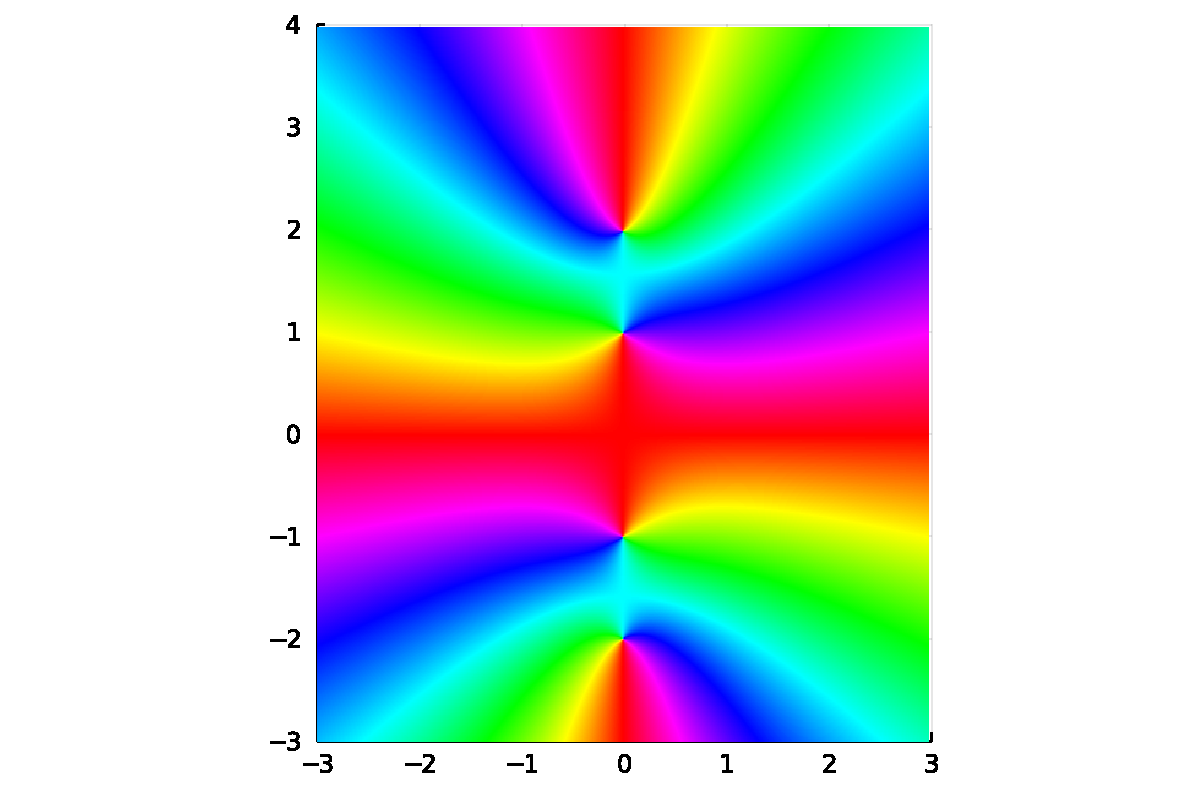
\includegraphics[width=\linewidth]{C:/Users/mfaso/OneDrive/Documents/GitHub/M3M6AppliedComplexAnalysis/output/figures/Solutions1_6_1.pdf}


\begin{align*}
	\int_{-\infty}^\infty    {1 \over (x^2+1)(x^2+4)} \dx &=
    2 \pi \I \left( \Res_{z = \I} + \Res_{z = 2\I}\right){1 \over (z^2+1)(z^2+4)} \\
    & = 2 \pi \I \left( {1 \over 2 \I 3 \I (-\I)} + {1 \over 3 \I  \I 4\I} \right) = \pi/ 6
\end{align*}
We can check the result numerically:


\begin{lstlisting}
(*@\HLJLn{x}@*) (*@\HLJLoB{=}@*) (*@\HLJLnf{Fun}@*)(*@\HLJLp{(}@*) (*@\HLJLnf{Line}@*)(*@\HLJLp{())}@*)
(*@\HLJLnf{sum}@*)(*@\HLJLp{(}@*)(*@\HLJLni{1}@*)(*@\HLJLoB{/}@*)(*@\HLJLp{((}@*)(*@\HLJLn{x}@*)(*@\HLJLoB{{\textasciicircum}}@*)(*@\HLJLni{2}@*)(*@\HLJLoB{+}@*)(*@\HLJLni{1}@*)(*@\HLJLp{)}@*)(*@\HLJLoB{*}@*)(*@\HLJLp{(}@*)(*@\HLJLn{x}@*)(*@\HLJLoB{{\textasciicircum}}@*)(*@\HLJLni{2}@*)(*@\HLJLoB{+}@*)(*@\HLJLni{4}@*)(*@\HLJLp{))),}@*) (*@\HLJLn{\ensuremath{\pi}}@*)(*@\HLJLoB{/}@*)(*@\HLJLni{6}@*)
\end{lstlisting}

\begin{lstlisting}
(0.5235987755982988, 0.5235987755982988)
\end{lstlisting}


\subsubsection{4.}
Again, decays like $O(z^{-2})$ in upper half plane so we can use residue calculus. This integrand has poles at $z = \I$ and $z = 3 \I$:


\begin{lstlisting}
(*@\HLJLnf{phaseplot}@*)(*@\HLJLp{(}@*)(*@\HLJLoB{-}@*)(*@\HLJLnfB{4..4}@*)(*@\HLJLp{,}@*) (*@\HLJLoB{-}@*)(*@\HLJLnfB{4..4}@*)(*@\HLJLp{,}@*) (*@\HLJLn{z}@*)(*@\HLJLoB{->}@*) (*@\HLJLp{(}@*)(*@\HLJLn{z}@*)(*@\HLJLoB{{\textasciicircum}}@*)(*@\HLJLni{2}@*) (*@\HLJLoB{-}@*) (*@\HLJLn{z}@*) (*@\HLJLoB{+}@*) (*@\HLJLni{2}@*)(*@\HLJLp{)}@*) (*@\HLJLoB{/}@*) (*@\HLJLp{(}@*)(*@\HLJLn{z}@*)(*@\HLJLoB{{\textasciicircum}}@*)(*@\HLJLni{4}@*) (*@\HLJLoB{+}@*) (*@\HLJLni{10}@*)(*@\HLJLn{z}@*)(*@\HLJLoB{{\textasciicircum}}@*)(*@\HLJLni{2}@*) (*@\HLJLoB{+}@*)(*@\HLJLni{9}@*)(*@\HLJLp{))}@*)
\end{lstlisting}

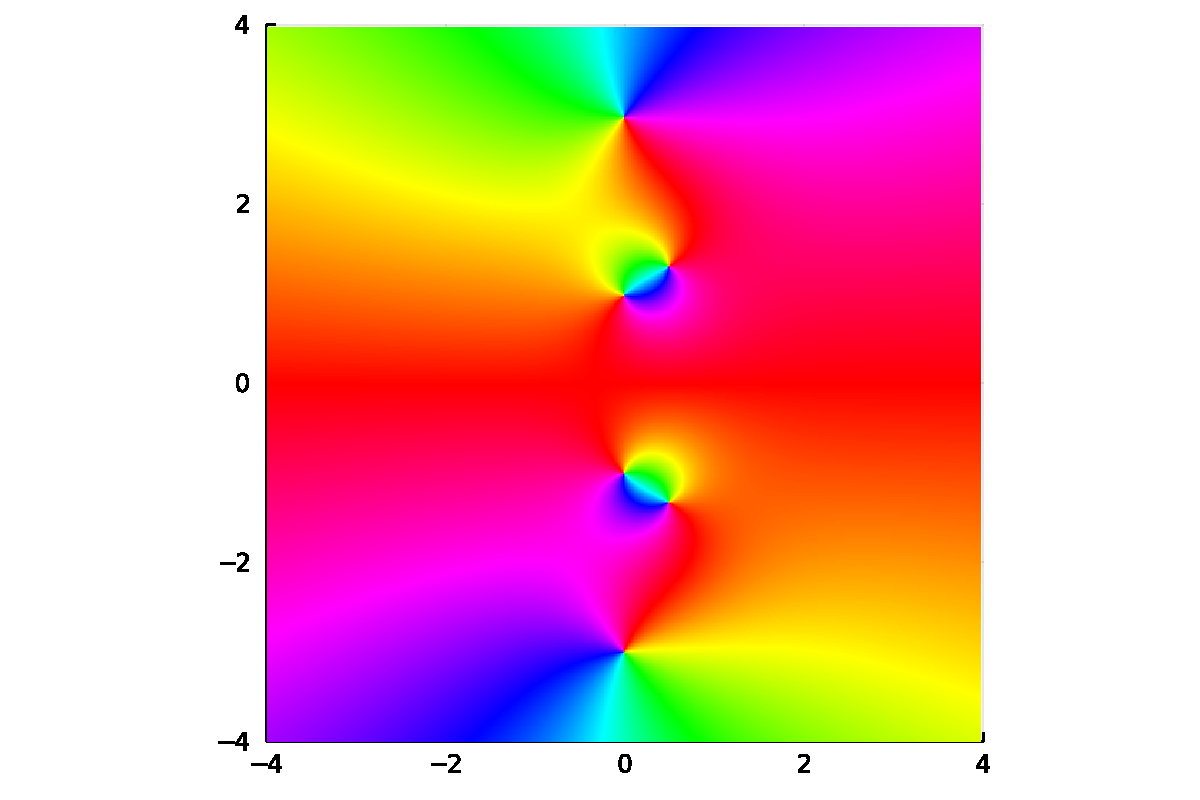
\includegraphics[width=\linewidth]{C:/Users/mfaso/OneDrive/Documents/GitHub/M3M6AppliedComplexAnalysis/output/figures/Solutions1_8_1.pdf}

The residues are $(-1-\I)/16$ and $(3-7\I)/48$ giving the answer

\[
5\pi \over 12
\]
which we check numerically:


\begin{lstlisting}
(*@\HLJLn{f}@*) (*@\HLJLoB{=}@*) (*@\HLJLn{x}@*) (*@\HLJLoB{->}@*) (*@\HLJLp{(}@*)(*@\HLJLn{x}@*)(*@\HLJLoB{{\textasciicircum}}@*)(*@\HLJLni{2}@*) (*@\HLJLoB{-}@*) (*@\HLJLn{x}@*) (*@\HLJLoB{+}@*) (*@\HLJLni{2}@*)(*@\HLJLp{)}@*) (*@\HLJLoB{/}@*) (*@\HLJLp{(}@*)(*@\HLJLn{x}@*)(*@\HLJLoB{{\textasciicircum}}@*)(*@\HLJLni{4}@*) (*@\HLJLoB{+}@*) (*@\HLJLni{10}@*)(*@\HLJLn{x}@*)(*@\HLJLoB{{\textasciicircum}}@*)(*@\HLJLni{2}@*) (*@\HLJLoB{+}@*)(*@\HLJLni{9}@*)(*@\HLJLp{)}@*)
(*@\HLJLnf{sum}@*)(*@\HLJLp{(}@*)(*@\HLJLnf{Fun}@*)(*@\HLJLp{(}@*)(*@\HLJLn{f}@*)(*@\HLJLp{,}@*)(*@\HLJLoB{-}@*)(*@\HLJLnfB{10{\_}000..10{\_}000}@*)(*@\HLJLp{)),}@*) (*@\HLJLni{5}@*)(*@\HLJLn{\ensuremath{\pi}}@*)(*@\HLJLoB{/}@*)(*@\HLJLni{12}@*)
\end{lstlisting}

\begin{lstlisting}
(1.3087969390010812, 1.3089969389957472)
\end{lstlisting}


\subsubsection{5.}
\[
	\int_{-\infty}^\infty    {1 \over x + \I } \dx
\]
Trick question: it's undefined because the integral doesn't decay fast enough. But what if I had asked for

\[
	\dashint_{-\infty}^\infty    {1 \over x + \I } \dx?
\]
We can't use residue theorem since it doesn't decay fast enough, but we can use, with a contour $C_R = \{ R \E^{\I \theta} : 0 \leq \theta \leq \pi \}$

\[
\oint_{[-M, M] \cup C_R} {1 \over z + \I}   = 0
\]
Further, by direct substitution, we have

\[
\int_{C_R} {1 \over z + \I}\dz = \I \int_0^\pi  R {\E^{\I \theta} \over R \E^{\I \theta} + \I} \D \theta
\]
Letting $R \rightarrow \infty$, the integrand tends to one uniformly hence

\[
 \int_{C_R} {1 \over z + \I}\dz  \rightarrow \I \int_0^\pi  \D \theta  = \I \pi.
\]
Therefore, we have

\[
	\dashint_{-\infty}^\infty    {1 \over x + \I } \dx = \lim_{M\rightarrow \infty} \int_{-M}^M {1 \over x + \I}  \dx =  - \I \pi .
\]
\begin{verbatim}
Indeed:
\end{verbatim}

\begin{lstlisting}
(*@\HLJLn{x}@*) (*@\HLJLoB{=}@*) (*@\HLJLnf{Fun}@*)(*@\HLJLp{(}@*)(*@\HLJLoB{-}@*)(*@\HLJLni{1000}@*) (*@\HLJLoB{..}@*) (*@\HLJLni{1000}@*)(*@\HLJLp{)}@*)
(*@\HLJLnf{sum}@*)(*@\HLJLp{(}@*)(*@\HLJLni{1}@*)(*@\HLJLoB{/}@*)(*@\HLJLp{(}@*)(*@\HLJLn{x}@*)(*@\HLJLoB{+}@*)(*@\HLJLn{im}@*)(*@\HLJLp{))}@*)
\end{lstlisting}

\begin{lstlisting}
1.1102230246251565e-15 - 3.1395926542565897im
\end{lstlisting}


\subsubsection{6.}
\[
\int_{-\infty}^\infty    {\sin 2x \over x^2 + x + 1} \dx = \Im \int_{-\infty}^\infty    {\E^{ 2 \I x} \over x^2 + x + 1} \dx
\]
This can be deformed in the upper half plane with a pole at ${-1 + \I \sqrt{3} \over 2}$, using residue calculus gives us

\[
   -{2 \pi \over \sqrt 3} {\sin 1 \over \E^{\sqrt{3}}}
\]

\begin{lstlisting}
(*@\HLJLn{x}@*) (*@\HLJLoB{=}@*) (*@\HLJLnf{Fun}@*)(*@\HLJLp{(}@*)(*@\HLJLoB{-}@*)(*@\HLJLni{100}@*) (*@\HLJLoB{..}@*) (*@\HLJLni{100}@*)(*@\HLJLp{)}@*)
(*@\HLJLnf{sum}@*)(*@\HLJLp{(}@*)(*@\HLJLnf{sin}@*)(*@\HLJLp{(}@*)(*@\HLJLni{2}@*)(*@\HLJLn{x}@*)(*@\HLJLp{)}@*)(*@\HLJLoB{/}@*)(*@\HLJLp{(}@*)(*@\HLJLn{x}@*)(*@\HLJLoB{{\textasciicircum}}@*)(*@\HLJLni{2}@*)(*@\HLJLoB{+}@*)(*@\HLJLn{x}@*)(*@\HLJLoB{+}@*)(*@\HLJLni{1}@*)(*@\HLJLp{)),}@*)(*@\HLJLoB{-}@*)(*@\HLJLni{2}@*)(*@\HLJLn{\ensuremath{\pi}}@*)(*@\HLJLoB{/}@*)(*@\HLJLnf{sqrt}@*)(*@\HLJLp{(}@*)(*@\HLJLni{3}@*)(*@\HLJLp{)}@*) (*@\HLJLoB{*}@*) (*@\HLJLnf{sin}@*)(*@\HLJLp{(}@*)(*@\HLJLni{1}@*)(*@\HLJLp{)}@*)(*@\HLJLoB{/}@*)(*@\HLJLnf{exp}@*)(*@\HLJLp{(}@*)(*@\HLJLnf{sqrt}@*)(*@\HLJLp{(}@*)(*@\HLJLni{3}@*)(*@\HLJLp{))}@*)
\end{lstlisting}

\begin{lstlisting}
(-0.5400548830723215, -0.5400553569742235)
\end{lstlisting}


\subsubsection{7.}
\[
	\int_{-\infty}^\infty    {\cos x \over x^2 + 4} \dx = \Re 	\int_{-\infty}^\infty    {\E^{\I x}\over x^2 + 4} \dx
\]
and residue calculus gives ${\pi \over 2 \E^2}$


\begin{lstlisting}
(*@\HLJLn{M}@*) (*@\HLJLoB{=}@*) (*@\HLJLni{200}@*)
(*@\HLJLn{x}@*) (*@\HLJLoB{=}@*) (*@\HLJLnf{Fun}@*)(*@\HLJLp{(}@*)(*@\HLJLoB{-}@*)(*@\HLJLn{M}@*) (*@\HLJLoB{..}@*) (*@\HLJLn{M}@*)(*@\HLJLp{)}@*)
(*@\HLJLnf{sum}@*)(*@\HLJLp{(}@*)(*@\HLJLnf{cos}@*)(*@\HLJLp{(}@*)(*@\HLJLn{x}@*)(*@\HLJLp{)}@*)(*@\HLJLoB{/}@*)(*@\HLJLp{(}@*)(*@\HLJLn{x}@*)(*@\HLJLoB{{\textasciicircum}}@*)(*@\HLJLni{2}@*)(*@\HLJLoB{+}@*)(*@\HLJLni{4}@*)(*@\HLJLp{)),}@*)(*@\HLJLn{\ensuremath{\pi}}@*)(*@\HLJLoB{/}@*)(*@\HLJLp{(}@*)(*@\HLJLni{2}@*)(*@\HLJLoB{*}@*)(*@\HLJLnf{exp}@*)(*@\HLJLp{(}@*)(*@\HLJLni{2}@*)(*@\HLJLp{))}@*) (*@\HLJLcs{{\#}}@*) (*@\HLJLcs{converges}@*) (*@\HLJLcs{if}@*) (*@\HLJLcs{we}@*) (*@\HLJLcs{make}@*) (*@\HLJLcs{M}@*) (*@\HLJLcs{even}@*) (*@\HLJLcs{bigger}@*)
\end{lstlisting}

\begin{lstlisting}
(0.21254026836701112, 0.21258416579381814)
\end{lstlisting}


\subsubsection{8.}
\[
	\int_{-\infty}^\infty    {x \sin x \over x^2 + 1} \dx = { \pi \over \E}
\]
using Residue calculus. You need to appeal to Jordan's lemma to argue that it can still be done even with only $O(x^{-1})$ decay.


\begin{lstlisting}
(*@\HLJLn{M}@*) (*@\HLJLoB{=}@*) (*@\HLJLni{10{\_}000}@*)
(*@\HLJLn{x}@*) (*@\HLJLoB{=}@*) (*@\HLJLnf{Fun}@*)(*@\HLJLp{(}@*)(*@\HLJLoB{-}@*)(*@\HLJLn{M}@*) (*@\HLJLoB{..}@*) (*@\HLJLn{M}@*)(*@\HLJLp{)}@*)
(*@\HLJLnf{sum}@*)(*@\HLJLp{(}@*)(*@\HLJLn{x}@*)(*@\HLJLoB{*}@*)(*@\HLJLnf{sin}@*)(*@\HLJLp{(}@*)(*@\HLJLn{x}@*)(*@\HLJLp{)}@*)(*@\HLJLoB{/}@*)(*@\HLJLp{(}@*)(*@\HLJLn{x}@*)(*@\HLJLoB{{\textasciicircum}}@*)(*@\HLJLni{2}@*)(*@\HLJLoB{+}@*)(*@\HLJLni{1}@*)(*@\HLJLp{)),}@*)(*@\HLJLn{\ensuremath{\pi}}@*)(*@\HLJLoB{/}@*)(*@\HLJLnf{exp}@*)(*@\HLJLp{(}@*)(*@\HLJLni{1}@*)(*@\HLJLp{)}@*) (*@\HLJLcs{{\#}}@*) (*@\HLJLcs{Converges}@*) (*@\HLJLcs{if}@*) (*@\HLJLcs{we}@*) (*@\HLJLcs{make}@*) (*@\HLJLcs{M}@*) (*@\HLJLcs{even}@*) (*@\HLJLcs{bigger}@*)
\end{lstlisting}

\begin{lstlisting}
(1.1559177936504117, 1.1557273497909217)
\end{lstlisting}


\subsubsection{9.}
\[
\int_{-\infty}^\infty {\cos a x - \cos b x \over x^2}  \dx \qqwhere a,b > 0
\]
We have for $f(x) = {\E^{\I a x} - \E^{\I b x} \over x^2}$

\[
\Re f(x) = {\cos a x - \cos b x \over x^2}
\]
Note that, since $\cos x = 1 + x^2/2 + O(x^4)$, the integrand is fine near zero:

\[
{\cos a x - \cos b x \over x^2} = {(a -b)  \over 2} + O(x^2)
\]
But $f(x)$ has a pole:

\[
     {\E^{\I a x} - \E^{\I b x} \over x^2}  = {\I (a-b) \over x} + O(1)
\]
To rectify this, we need to be a bit more careful. First note that

\[
\int_{\infty}^\infty {\cos a x - \cos b x \over x^2} \dx = \lim_{\epsilon \rightarrow 0} \left(\int_{-\infty}^{-\epsilon} + \int_\epsilon^\infty \right){\cos a x - \cos b x \over x^2} \dx = \Re \dashint_{-\infty}^\infty f(x) \dx
\]
Then we construct a contour avoiding zero as follows:


\begin{lstlisting}
(*@\HLJLn{M}@*) (*@\HLJLoB{=}@*) (*@\HLJLni{10}@*)
(*@\HLJLn{\ensuremath{\varepsilon}}@*) (*@\HLJLoB{=}@*) (*@\HLJLnfB{1.0}@*)

(*@\HLJLnf{plot}@*)(*@\HLJLp{(}@*)(*@\HLJLnf{Segment}@*)(*@\HLJLp{(}@*)(*@\HLJLoB{-}@*)(*@\HLJLn{M}@*)(*@\HLJLp{,}@*) (*@\HLJLoB{-}@*)(*@\HLJLn{\ensuremath{\varepsilon}}@*)(*@\HLJLp{)}@*) (*@\HLJLoB{\ensuremath{\cup}}@*) (*@\HLJLnf{Segment}@*)(*@\HLJLp{(}@*)(*@\HLJLn{\ensuremath{\varepsilon}}@*)(*@\HLJLp{,}@*) (*@\HLJLn{M}@*)(*@\HLJLp{);}@*)(*@\HLJLn{label}@*)(*@\HLJLoB{=}@*)(*@\HLJLs{"{}[-M,e]}@*) (*@\HLJLs{U}@*) (*@\HLJLs{[e,M]"{}}@*)(*@\HLJLp{,}@*) (*@\HLJLn{ratio}@*) (*@\HLJLoB{=}@*) (*@\HLJLnfB{1.0}@*)(*@\HLJLp{)}@*)
(*@\HLJLnf{plot!}@*)(*@\HLJLp{(}@*)(*@\HLJLnf{Arc}@*)(*@\HLJLp{(}@*)(*@\HLJLnfB{0.}@*)(*@\HLJLp{,}@*)(*@\HLJLn{\ensuremath{\varepsilon}}@*)(*@\HLJLp{,}@*) (*@\HLJLp{(}@*)(*@\HLJLn{\ensuremath{\pi}}@*)(*@\HLJLp{,}@*)(*@\HLJLnfB{0.}@*)(*@\HLJLp{));}@*) (*@\HLJLn{label}@*)(*@\HLJLoB{=}@*)(*@\HLJLs{"{}C{\_}e"{}}@*)(*@\HLJLp{)}@*)
(*@\HLJLnf{plot!}@*)(*@\HLJLp{(}@*)(*@\HLJLnf{Arc}@*)(*@\HLJLp{(}@*)(*@\HLJLnfB{0.}@*)(*@\HLJLp{,}@*) (*@\HLJLn{M}@*)(*@\HLJLp{,}@*) (*@\HLJLp{(}@*)(*@\HLJLni{0}@*)(*@\HLJLp{,}@*)(*@\HLJLn{\ensuremath{\pi}}@*)(*@\HLJLp{));}@*) (*@\HLJLn{label}@*) (*@\HLJLoB{=}@*) (*@\HLJLs{"{}C{\_}M"{}}@*)(*@\HLJLp{)}@*)
\end{lstlisting}

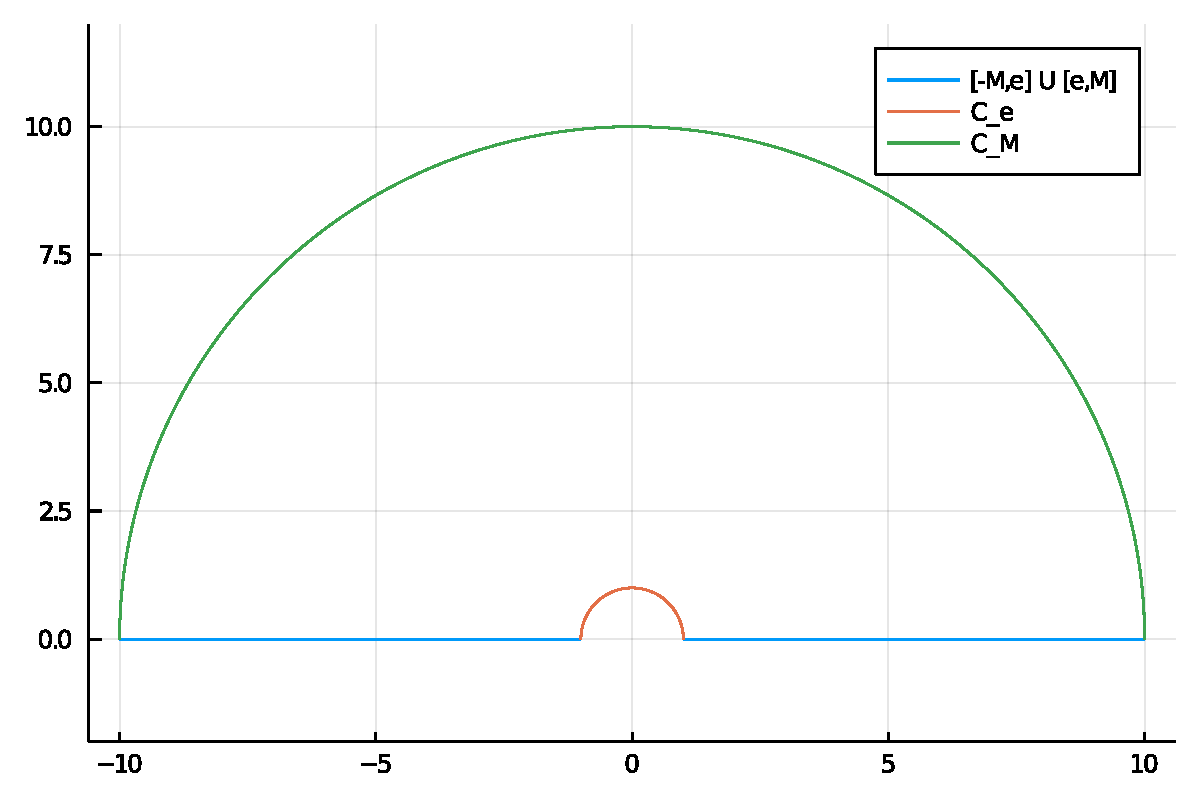
\includegraphics[width=\linewidth]{C:/Users/mfaso/OneDrive/Documents/GitHub/M3M6AppliedComplexAnalysis/output/figures/Solutions1_14_1.pdf}

Note that $\oint_\gamma f(z) \dz = 0$,

\[
\int_{C_\epsilon} {\E^{\I a z } - \E^{\I b z} \over z^2} \dz =
 \int_\pi^0 { (b-a) \E^{\I \theta}  + O(\epsilon) \over \E^{ \I \theta}} \D\theta \rightarrow (a-b) \pi
\]
Also, as the integrand is $O(z^{-2})$ the integral over $C_M$ vanishes as $M \rightarrow \infty$. We therefore get

\[
    \dashint f(x)\dx = (b-a)\pi
\]

\begin{lstlisting}
(*@\HLJLn{\ensuremath{\varepsilon}}@*) (*@\HLJLoB{=}@*)(*@\HLJLnfB{0.001}@*)
(*@\HLJLn{M}@*) (*@\HLJLoB{=}@*) (*@\HLJLnfB{1{\_}000.0}@*)
(*@\HLJLn{x}@*) (*@\HLJLoB{=}@*) (*@\HLJLnf{Fun}@*)(*@\HLJLp{(}@*)(*@\HLJLnf{Segment}@*)(*@\HLJLp{(}@*)(*@\HLJLoB{-}@*)(*@\HLJLn{M}@*) (*@\HLJLp{,}@*) (*@\HLJLoB{-}@*)(*@\HLJLn{\ensuremath{\varepsilon}}@*)(*@\HLJLp{)}@*) (*@\HLJLoB{\ensuremath{\cup}}@*) (*@\HLJLnf{Segment}@*)(*@\HLJLp{(}@*)(*@\HLJLn{\ensuremath{\varepsilon}}@*)(*@\HLJLp{,}@*) (*@\HLJLn{M}@*)(*@\HLJLp{))}@*)
(*@\HLJLn{a}@*) (*@\HLJLoB{=}@*) (*@\HLJLnfB{2.3}@*)(*@\HLJLp{;}@*) (*@\HLJLn{b}@*) (*@\HLJLoB{=}@*) (*@\HLJLnfB{3.8}@*)
(*@\HLJLnf{sum}@*)(*@\HLJLp{((}@*)(*@\HLJLnf{cos}@*)(*@\HLJLp{(}@*)(*@\HLJLn{a}@*)(*@\HLJLoB{*}@*)(*@\HLJLn{x}@*)(*@\HLJLp{)}@*) (*@\HLJLoB{-}@*) (*@\HLJLnf{cos}@*)(*@\HLJLp{(}@*)(*@\HLJLn{b}@*)(*@\HLJLoB{*}@*)(*@\HLJLn{x}@*)(*@\HLJLp{))}@*)(*@\HLJLoB{/}@*)(*@\HLJLn{x}@*)(*@\HLJLoB{{\textasciicircum}}@*)(*@\HLJLni{2}@*)(*@\HLJLp{),}@*)(*@\HLJLn{\ensuremath{\pi}}@*)(*@\HLJLoB{*}@*)(*@\HLJLp{(}@*)(*@\HLJLn{b}@*)(*@\HLJLoB{-}@*)(*@\HLJLn{a}@*)(*@\HLJLp{)}@*) (*@\HLJLcs{{\#}}@*) (*@\HLJLcs{Converges}@*) (*@\HLJLcs{if}@*) (*@\HLJLcs{we}@*) (*@\HLJLcs{make}@*) (*@\HLJLcs{M}@*) (*@\HLJLcs{bigger}@*)
\end{lstlisting}

\begin{lstlisting}
(4.703250780477666, 4.71238898038469)
\end{lstlisting}


\subsubsection{10.}
Use binomial formula


\begin{align*}
\int_0^{2 \pi} (\cos \theta)^n \D \theta &= {1 \over 2^n \I} \oint (z+z^{-1})^n {\dz \over z} \\
 &=  {1 \over 2^n \I} \sum_{k=0}^n {n! \over k! (n-k)!} \oint z^k z^{k-n} {\dz \over z} \\
 &=  {1 \over 2^n \I} \sum_{k=0}^n {n! \over k! (n-k)!} \oint z^{2k-n-1}\dz
\end{align*}
We only have a residue of $2k-n-1 = -1$, that is, if $2k = n$. If $n$ is odd, this can't happen (duh! the integral is symmetric with respect to $\theta$). If it's even, then we have

\[
\int_0^{2 \pi} (\cos \theta)^n \D \theta =  {\pi \over 2^{n-1} }  {n! \over  ((n/2)!)^2}
\]

\begin{lstlisting}
(*@\HLJLn{\ensuremath{\theta}}@*) (*@\HLJLoB{=}@*) (*@\HLJLnf{Fun}@*)(*@\HLJLp{(}@*)(*@\HLJLni{0}@*) (*@\HLJLoB{..}@*) (*@\HLJLni{2}@*)(*@\HLJLn{\ensuremath{\pi}}@*)(*@\HLJLp{)}@*)
(*@\HLJLn{n}@*) (*@\HLJLoB{=}@*) (*@\HLJLni{10}@*)(*@\HLJLp{;}@*)
(*@\HLJLnf{sum}@*)(*@\HLJLp{(}@*)(*@\HLJLnf{cos}@*)(*@\HLJLp{(}@*)(*@\HLJLn{\ensuremath{\theta}}@*)(*@\HLJLp{)}@*)(*@\HLJLoB{{\textasciicircum}}@*)(*@\HLJLn{n}@*)(*@\HLJLp{),}@*) (*@\HLJLn{\ensuremath{\pi}}@*)(*@\HLJLoB{*}@*)(*@\HLJLnf{factorial}@*)(*@\HLJLp{(}@*)(*@\HLJLnfB{1.0}@*)(*@\HLJLn{n}@*)(*@\HLJLp{)}@*)(*@\HLJLoB{/}@*)(*@\HLJLp{(}@*)(*@\HLJLni{2}@*)(*@\HLJLoB{{\textasciicircum}}@*)(*@\HLJLp{(}@*)(*@\HLJLn{n}@*)(*@\HLJLoB{-}@*)(*@\HLJLni{1}@*)(*@\HLJLp{)}@*)(*@\HLJLoB{*}@*)(*@\HLJLnf{factorial}@*)(*@\HLJLp{(}@*)(*@\HLJLn{n}@*)(*@\HLJLoB{/}@*)(*@\HLJLni{2}@*)(*@\HLJLp{)}@*)(*@\HLJLoB{{\textasciicircum}}@*)(*@\HLJLni{2}@*)(*@\HLJLp{)}@*)
\end{lstlisting}

\begin{lstlisting}
(1.5462526341887322, 1.5462526341887264)
\end{lstlisting}


\subsection{Problem 2.1}
By integrating around a rectangular contour with vertices at $\pm R$ and $\pi \I \pm R$ and letting $R \rightarrow \infty$, show that:

\[
\int_0^\infty \sech x \dx = {\pi \over 2}
\]
where $\sech x = {2 \over \E^{-x} + \E^x}$.

Recall $\sech x = {2 \over \E^{-x} + \E^x} $. This shows that $\sech(-x) = \sech x$ But we also have

\[
\sech(x + \I \pi) =  {2 \over \E^{-x-\I \pi} + \E^{x+ \I \pi}} =  {2 \over -\E^{-x} - \E^{x}} = -\sech x
\]
Thus we have

\[
    4\int_0^\infty \sech x \dx = \left[ \int_{-\infty}^\infty + \int_{\infty+\I\pi}^{-\infty + \I \pi} \right] \sech z \dz
\]
We can approximate this using

\[
\left[ \int_{-R}^R + \int_R^{R+\I \pi} + \int_{R+\I \pi}^{-R+\I\pi} + \int_{-R+\I \pi}^{-R} \right ] \sech z \dz = 2 \pi \I \Res_{z = {\I \pi \over 2}} \sech z  = 2 \pi
\]
since, for $z_0 = {\I \pi \over 2}$, we have

\[
\sech z = {1 \over \cos \I z} = {1 \over - \I \sin \I z_0 (z- z_0) + O(z-z_0)^2}
= -{\I \over (z- z_0)} + O(1)
\]
Finally, we need to show that the limit as $R \rightarrow \infty$ tends to the right value. In this case, it follows since

\[
 \left|\int_R^{R+\I \pi} \sech z \dz \right| \leq {2 \pi \E^{-R} \over 1 - \E^{-2R}} \rightarrow 0
\]
(and by symmetry for $\int_{-R+\I \pi}^{-R}$.)

\subsection{Problem 2.2}
Show that the Fourier transform of $\sech x$ satisfies

\[
\int_{-\infty}^\infty \E^{\I k x } \sech x \dx = \pi \sech {\pi k \over 2}
\]
Define

\[
f(z) = \E^{\I k z } \sech z = {2 \E^{(1+\I k) z} \over \E^{2 z } + 1}
\]
In this case, we have the symmetry

\[
f(x + \I \pi) = - \E^{- k \pi} \E^{\I k x} \sech x = - \E^{-k \pi} f(x)
\]

\begin{lstlisting}
(*@\HLJLn{k}@*) (*@\HLJLoB{=}@*) (*@\HLJLnfB{2.0}@*)
(*@\HLJLn{f}@*) (*@\HLJLoB{=}@*) (*@\HLJLn{z}@*) (*@\HLJLoB{->}@*) (*@\HLJLnf{exp}@*)(*@\HLJLp{(}@*)(*@\HLJLn{im}@*)(*@\HLJLoB{*}@*)(*@\HLJLn{k}@*)(*@\HLJLoB{*}@*)(*@\HLJLn{z}@*)(*@\HLJLp{)}@*)(*@\HLJLoB{*}@*)(*@\HLJLnf{sech}@*)(*@\HLJLp{(}@*)(*@\HLJLn{z}@*)(*@\HLJLp{)}@*)
(*@\HLJLoB{-}@*)(*@\HLJLnf{exp}@*)(*@\HLJLp{(}@*)(*@\HLJLoB{-}@*)(*@\HLJLn{k}@*)(*@\HLJLoB{*}@*)(*@\HLJLn{\ensuremath{\pi}}@*)(*@\HLJLp{)}@*)(*@\HLJLnf{f}@*)(*@\HLJLp{(}@*)(*@\HLJLnfB{2.0}@*)(*@\HLJLp{),}@*)(*@\HLJLnf{f}@*)(*@\HLJLp{(}@*)(*@\HLJLnfB{2.0}@*)(*@\HLJLoB{+}@*)(*@\HLJLn{im}@*)(*@\HLJLoB{*}@*)(*@\HLJLn{\ensuremath{\pi}}@*)(*@\HLJLp{)}@*)
\end{lstlisting}

\begin{lstlisting}
(0.00032444937189257726 + 0.0003756543878221788im, 0.0003244493718925772 + 
0.00037565438782217884im)
\end{lstlisting}


In other words, we have

\[
(1 + \E^{-k \pi}) \int_{-\infty}^\infty f(x) \dx =\left(\int_{-\infty}^\infty +  \int_{\infty+\I \pi}^{-\infty + \I \pi}\right) f(z) \dz
\]
By similar logic as above, we can show that the integral over the rectangular contour converges to this.

Again, the only pole inside is at $z = {\I \pi \over 2}$, where the residue is $-\I \E^{-\pi k \over 2}$. Thus we have

\[
\int_{-\infty}^\infty f(x) \dx = {2 \pi \E^{-\pi k \over 2} \over 1 + \E^{-k \pi}} = \pi \sech{\pi k \over 2}
\]


\end{document}
